\documentclass[onlytextwidth]{beamer}
\usepackage[utf8]{inputenc}
\usepackage{microtype}
\usepackage{amsmath}
\usepackage{amssymb}
\usepackage[nomessages]{fp} %\FPeval{\var-name}{2*sin(pi/6)}
\usepackage{siunitx} %units in math. eg 20\milli\meter
\usepackage{yhmath} % for arcs, overparenth command
\usepackage{tikz} %graphics
\usetikzlibrary{quotes, angles}
%\usepackage{graphicx} already loaded by beamer class
%consider setting \graphicspath{{images/}}
%\parskip ?? to avoid paragraph indent
\usepackage{multicol} %may not need this package, just columns environment
\usepackage{venndiagram}

\subtitle[BECA]{Bronx Early College Academy}
\author[Huson]{Christopher J. Huson PhD}

\setbeamertemplate{headline}{\vskip2mm 
  BECA / \insertshortauthor \, / \inserttitle
  \hfill 
  \insertsection
  }

\title{Geometry Unit 1, part b: Area}
\date{19-23 September 2022}

\begin{document}
\frame{\titlepage}

\section[Outline]{}
\frame{\tableofcontents}

\section{1.8 Area \hfill 19 September}
\begin{frame}{Learning Target: I can calculate areas}
  {CCSS: HSG.CO.A.1 Know precise geometric definitions \hfill \alert{1.8 Monday 19 Sept}}
  \begin{block}{Do Now: Practice unit conversion}
    \begin{enumerate}
        \item How many days are in a week?
        \item Find the number of weeks in 365 days. \par (show calculation with units)
    \end{enumerate}
    \end{block} \vspace{3cm}
    Quiz results \par \medskip
    Lesson: Rectangle, triangle, parallelogram area formulas \par \medskip
    Extension: Scientific notation
  \end{frame}

\begin{frame}{The \emph{area} of a rectangle is its base $\times$ height.}
    {We also say ``length times width''}
    Formula for the area of a rectangle:
    {\large $$A=b \times h$$}
        \begin{columns}
            \column{0.5\textwidth}
            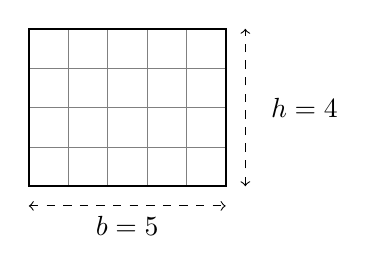
\begin{tikzpicture}[scale=.5]
                \draw[help lines] (0,0) grid (5,4);
                \draw[thick] (0,0)--(5,0)--(5,4)--(0,4)--cycle;
                \draw[<->, dashed] (0,-0.5)--(5,-0.5);
                \node at (2.5, -1){$b=5$};
                \draw[<->, dashed] (5.5,0)--(5.5,4);
                \node at (7, 2){$h=4$};
            \end{tikzpicture}
            \column{0.5\textwidth}
            $$A = 5 \times 4 = 20$$
        \end{columns} \vspace{1.5cm}
        \begin{description}
            \item[Area] the quantity of unit squares that fill a shape
        \end{description}
    \end{frame}

\begin{frame}{A parallelogram's area has the same formula as a rectangle.}
    {Use the height, not the length of the slanted side.}
    Formula for the area of a parallelogram:
    {\large $$A=b \times h$$}
        \begin{columns}
            \column{0.5\textwidth}
            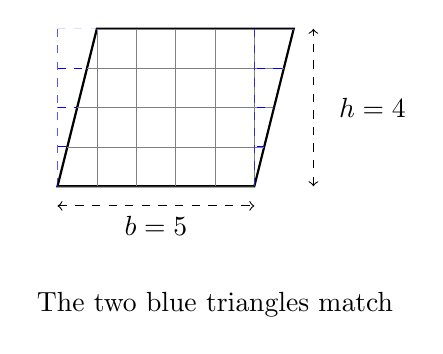
\begin{tikzpicture}[scale=.5]
                \draw[thick] (0,0)--(5,0)--(6,4)--(1,4)--cycle;
                \draw[<->, dashed] (0,-0.5)--(5,-0.5);
                \node at (2.5, -1){$b=5$};
                \draw[<->, dashed] (6.5,0)--(6.5,4);
                \node at (8, 2){$h=4$};
                \begin{scope}
                    \clip (0,0)--(5,0)--(6,4)--(1,4)--cycle;
                        \draw[help lines] (0,0) grid (6,4);
                \end{scope}
                \onslide<2>
                    \begin{scope}
                        \clip (0,0)--(1,4)--(0,4)--cycle;
                        \draw[dashed, blue] (0,0) grid (6,4);
                    \end{scope}
                    \begin{scope}
                        \clip (5,0)--(6,4)--(5,4)--cycle;
                        \draw[dashed, blue] (0,0) grid (6,4);
                    \end{scope}
                    \node at (4,-3){The two blue triangles match};
            \end{tikzpicture}
            \column{0.5\textwidth}
            $$A = 5 \times 4 = 20$$
        \end{columns} \vspace{1.5cm}
    \end{frame}

\begin{frame}{A triangle has half the area of its base times height.}
    {Use the height, not the side length.}
    Formula for the area of a triangle:
    {\large $$A= \frac{1}{2} b \times h$$}
        \begin{columns}
            \column{0.5\textwidth}
            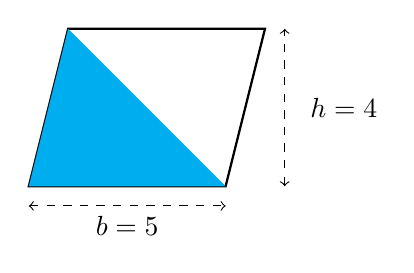
\begin{tikzpicture}[scale=.5]
                \draw[thick] (0,0)--(5,0)--(6,4)--(1,4)--cycle;
                \draw[<->, dashed] (0,-0.5)--(5,-0.5);
                \node at (2.5, -1){$b=5$};
                \draw[<->, dashed] (6.5,0)--(6.5,4);
                \node at (8, 2){$h=4$};
                \fill [cyan] (0,0)--(5,0)--(1,4)--cycle;
            \end{tikzpicture}
            \column{0.5\textwidth}
            $$A =  \frac{1}{2} (5 \times 4) = 10$$
        \end{columns} \vspace{1.5cm}
    \end{frame}

\begin{frame}{Find a missing dimension using the area formula}
    Given the area of a triangle is 40 and its base is 10, find its height. \vspace{1cm}
    \begin{columns}
        \column{0.5\textwidth}
        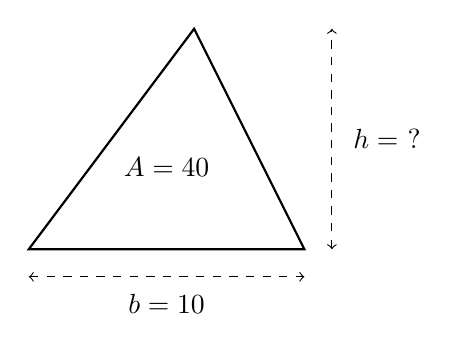
\begin{tikzpicture}[scale=.7]
            \draw[thick] (0,0)--(5,0)--(3,4)--cycle;
            \draw[<->, dashed] (0,-0.5)--(5,-0.5);
            \node at (2.5,-1){$b=10$};
            \draw[<->, dashed] (5.5,0)--(5.5,4);
            \node at (6.5,2){$h=$ ?};
            \node at (2.5,1.5){$A=40$};
        \end{tikzpicture}
        \column{0.5\textwidth}
        $$A =  \frac{1}{2} (10 \times h) = 40$$
    \end{columns} \vspace{1.5cm}
    \end{frame}

\begin{frame}{Write formulas in notebook}
        \begin{description}
            \item[Rectangle] $A=b \times h$ (base times height or length times width)
            \item[Parallelogram] $A=b \times h$
            \item[Triangle] $A=\frac{1}{2} (b \times h)$ \vspace{0.5cm}
            \item[Area] the quantity of unit squares that fill a shape
            \item[Units] We say ``square units'', i.e. square inches (abbreviated $\rm{in}^2$), square miles, etc.
        \end{description}
    \end{frame}
    
\section{1.9 Rounding and circle area \hfill 20 September}
\begin{frame}{Learning Target: I can calculate the area of a circle}
    {CCSS: HSG.CO.A.1 Know precise geometric definitions \hfill \alert{1.9 Tuesday 20 Sept}}
        Do Now: Two rectangles are shown. Calculate the area of each and the combined total area.
        \begin{flushleft}
            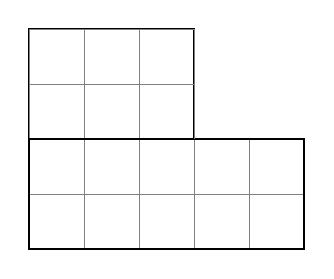
\begin{tikzpicture}[scale=.7]
                \draw[help lines] (0,0) grid (5,2);
                \draw[thick] (0,0)--(5,0)--(5,2)--(3,2)--(3,4)--(0,4)--cycle;
                \draw[help lines] (0,2) grid (3,4);
                \draw[thick] (0,2)--(3,2);
            \end{tikzpicture}
          \end{flushleft}
        Lesson: Area of a circle, $\pi$, decimals, powers of ten, rounding \par \medskip
        Extension: Significant figures
    \end{frame}

\section{1.10 Precision \hfill 21 September}
\begin{frame}{Learning Target: I can quantify error in calculations}
    {CCSS: HSG.CO.A.1 Know precise geometric definitions \hfill \alert{1.10 Wednesday 21 Sept}}
        Do Now: Find the area of a circle with radius $b=10$ centimeters, rounding to the nearest whole number. \par
        circle image \\

        Lesson: Percent error formula \par \medskip
        Extension: Confidence intervals
    \end{frame}  

\section{1.11 Review \hfill 22 September}
\begin{frame}{Learning Target: I can study together with my classmates}
    {CCSS: HSG.CO.A.1 Know precise geometric definitions \hfill \alert{1.11 Thursday 22 Sept}}
        Do Now: Find the area of a circle with radius $b=10$ centimeters, rounding to the nearest whole number. \par
        circle image \\

        Lesson: Peer review, notebook check, homework inventory due \par \medskip
        \alert{Unit test tomorrow}
    \end{frame} 

\begin{frame}{Groupwork review for \alert{test tomorrow}}
    {``Roundtable'' of four students, with four topics assigned}
    \begin{block}{Geometry skills to study / teach}
        \begin{enumerate}
        \item Conventions: terminology, notation, diagramming
        \item Modeling situations with algebra
        \item Perimeter and special shapes: 
        \begin{itemize}
        \item Scalene, isosceles, and equilateral $\triangle$s
        \item Squares, rectangles, parallelograms, trapezoids, rhombuses, kites \par 
        (quadrilateral side $\cong$s will be marked)
        \end{itemize}
        \item Solving algebraic equations for one variable
    \end{enumerate}
    \end{block}
    \end{frame}
    
\section{1.12 Unit test: Segments, length, area \hfill 23 September}
\begin{frame}{Learning Target: I can quantify length and area}
    {CCSS: HSG.CO.A.1 Know precise geometric definitions \hfill \alert{1.12 Friday 23 Sept}}

        \alert{Unit test}
    \end{frame} 
    
    
\end{document}